% -*- mode: latex-mode; TeX-engine: xetex; LaTeX-command-style: (("" "SOURCE_DATE_EPOCH=0 %(PDF)%(latex) --shell-escape %S%(PDFout)")); TeX-master: "../dissertation.tex"; -*-

\chapter{Photoassociation of Single Atoms}
\label{ch:pa}

\section{Introduction}

\todo{
  Need to measure the excited states in order to drive a two photon transition
  through the excited state.
  Define PA
  Mention size mismatch challenge.
}

\section{Energy Levels}

First we will discuss the energy levels in a diatomic molecule
as well as the labeling system for the states.
We will focus mainly on the electronic excited states measured in this chapter
but most of the discussion here applies to ground electronic states as well
and will be useful for chapter \label{ch:raman-spectroscopy} and \label{ch:raman-transfer}.

\subsection{Angular Momentums}

Compared to an atom, a diatomic molecule has many more degrees of freedoms.
In additional to the quantum numbers for each atom in the molecule,
molecules also have nuclear motion.
In order to reduce the complexity, it is therefore very important to consider the
symmetry of the system, and in particular the angular momentums,
which corresponds to rotation symmetry, and the coupling between them.
The angular momentums in a diatomic molecule includes electron orbit $\mathbf{L}$
\footnote{There are $\mathbf{L}_1$ and $\mathbf{L}_2$ for the two electron but since
  we only consider states with at most one $\mathbf{L}_i\neq0$ we will only use one quantum number here},
electron spin $\mathbf{S}_1$ and $\mathbf{S}_2$, nuclear orbital $\mathbf{N}$
and nuclear spin $\mathbf{I}_1$ and $\mathbf{I}_2$.
Although the total angular momentum
$\mathbf{F}\equiv\mathbf{L}+\mathbf{S}_1+\mathbf{S}_2+\mathbf{N}+\mathbf{I}_1+\mathbf{I}_2$
is the only true conserved quantity in the absence of external field,
depending on the coupling strengths between the angular momentums,
there are additional approximately conserved quantity in the molecule.

For the NaCs molecule and our experiment, there are two important regimes where the coupling
strength can be easily ordered.

\subsubsection{Deeply Bound States}

\begin{figure}
  \centering
  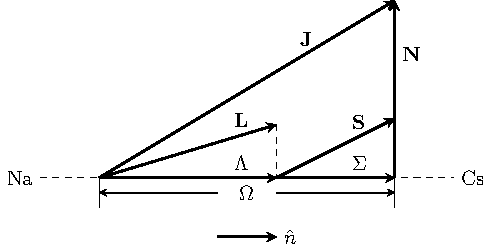
\includegraphics[width=\textwidth]{figures/pa_hunds_case_a.pdf}
  \caption[Hund's case (a)]{
    Angular momentum coupling for \textit{Hund's case (a)}.
    $\mathbf{L}$ and $\mathbf{S}$ are coupled to the internuclear axis $\hat n$
    and the sum of the projections $\Omega=\Lambda+\Sigma$ is then
    added with the orthogonal compoment $\mathbf{N}$ to form $\mathbf{J}$.
    \label{fig:pa-hunds-case-a}}
\end{figure}

This is described by the \textit{Hund's case (a)}.
Molecular states with large binding energies mostly experience interactions
between the atoms at short range where the electric static interaction is very strong.
This couples the the two electron spins into a total electron spin
$\mathbf{S}\equiv\mathbf{S}_1+\mathbf{S}_2$ via a very strong effective interaction
of the form $\mathbf{S}_1\cdot\mathbf{S}_2$ which originates
from the resulting symmetry of the electron orbital wavefunction.
Similar to atoms, the nuclear spin interaction is also very week compared to
other energy scales so we can ignore the hyperfine structure and only need to consider
$\mathbf{J}\equiv\mathbf{L}+\mathbf{S}+\mathbf{N}$.

The strong electrostatic interaction also creates an effective coupling
between the $\mathbf{L}$ and $\mathbf{S}$ with the internuclear axis $\hat{n}$
causing $\mathbf{L}$ and $\mathbf{S}$ to process rapidly around $\hat{n}$.
This creates two new conserved quantity $\Lambda$ and $\Sigma$
as the projection of $\mathbf{L}$ and $\mathbf{S}$
along $\hat{n}$ respectively.
The total angular momentum along $\hat{n}$ is therefore $\Omega\equiv\Lambda+\Sigma$
and it is added to the $\mathbf{N}$ which is orthogonal to $\hat{n}$ to form
the total angular momentum $\mathbf{J}$ (Fig~\ref{fig:pa-hunds-case-a}).

The angular momenum state of the molecule is therefore fully characterized by
$|L,\Lambda,S,\Omega,J\rangle$. $\Lambda$ can be $0,1,\dots,L$, $\Omega$ ranges from
$\abs{\Lambda-S}$ to $\Lambda+S$ and $J\geqslant\Omega$.
The $L$ quantum number is specified by the electronic state and will be discussed
in section \ref{ch:pa:pes} and the rest of the angular momentum quantum numbers
are represented by the \textit{Hund's case (a)} term symbol,
\[ ^{2S+1}\Lambda_\Omega \]
similar to the atomic term symbol $^{2S+1}L_J$.
Just as the use of capital English letters $S,P,D,\dots$ to represent
$L=0,1,2,\dots$, capital Greek letters $\Sigma,\Pi,\Delta,\dots$ are used
to denote $\Lambda=0,1,2,\dots$ in the term symbol.
An additional symmetry to consider is the reflection about a plane that includes
the internuclear axis.
For $\Lambda>0$ states, the reflection produces a new state at the same energy
creating the so-called $\Lambda$-doubling. For $\Lambda=0$ states, i.e. $\Sigma$ states,
the reflection produces the same state with a phase of $\pm1$.
This phase is also included in the term symbol to fully specify the symmetry of
a $\Sigma$ states as
\[ ^{2S+1}\Sigma_\Omega^{\pm} \]
Note the $\Sigma$ state here should not be confused with the quantum number $\Sigma$.

\todo{rotational energy? J(J+1) - Omega^2}

\subsubsection{Near Threshold Bound States}

For molecular states with small binding energy, the interaction between the two atoms is
small compared to the internal coupling in the atoms and
the angular momentum coupling is ``atom like''.
In this limit, the total angular momentum $\mathbf{F}_1$ and $\mathbf{F}_2$
for the individual atoms forms $\mathbf{F}_{atom}=\mathbf{F}_1+\mathbf{F}_2$
which is then coupled to the nuclear rotation $\mathbf{N}$
to form $\mathbf{F}=\mathbf{F}_{atom}+\mathbf{N}$.

\todo{mention N=2 spectroscopy?}

\subsection{Potential Energy Surface}
\label{ch:pa:pes}

Due to the different angular momentum coupling in different regimes,
there is not a consistent way to label the interaction between the two atoms
at both short and long distance.
Nevertheless, by convention, we use the \textit{Hund's case (a)} term symbol
since it more accurately represents the state when the interaction energy dominates.

The Hamiltonian (excluding spin for simplicity\footnote{Electron spin is implicitly included,
  however, via the symmetry of the electronic wavefunction.}) is,
\begin{align*}
  H=&H_e+T_n
\end{align*}
where the electronic term $H_e$ and the nuclear kinetic term $T_n$ are given by
\begin{align*}
  H_e=&-\sum_i\frac{\hbar}{2m_e}\mathbf{\nabla}_i^2+\frac{e^2}{4\pi\varepsilon_0}\paren{\sum_{i>j}\frac{1}{\abs{\mathbf{r}_i-\mathbf{r}_j}}-\sum_{A=Na,Cs}\sum_i\frac{Z_{A}}{\abs{\mathbf{r}_i-\mathbf{R}_{A}}}+\frac{Z_{Na}Z_{Cs}}{\abs{\mathbf{R}_{Cs}-\mathbf{R}_{Na}}}}\numberthis{eq:pa:pes:he}\\
  T_n=&-\sum_{A=Na,Cs}\frac{\hbar^2}{2m_{A}}\mathbf{\nabla}_{A}^2
\end{align*}
and the sum is over all the electrons in the molecule.

\subsubsection{Born-Oppenheimer Approximation}

The Hamiltonian is solved using the Born-Oppenheimer (BO) approximation.
Because of the large mass difference between the nuclei and the electrons,
we can assume that the electron motion follows the position of the nuclei
instantaneously so that the motion of the nuclei and the elctrons can be treated separately.
Formally, this mean that the electron wavefunctions is solved using the
electrionic term $H_e$ for a given nuclear position $\mathbf{R}_{Na}$ and $\mathbf{R}_{Cs}$.
This results in an effective potential $V_{eff}\paren{\abs{\mathbf{R}_{Na}-\mathbf{R}_{Cs}}}$ called
the potential energy surfaces (PES) for each electronic states.
The solutions to the approximate Hamiltonians $T_n+V_{eff}$ provide
the vibrational and rotational states of the molecule.

\subsubsection{Franck-Condon Factor}

In additional to the energy of the molecular bound state,
the solution of the nuclear motion also provides information to the selection rules
and coupling strength of transitions between the states.
For an electronic electric dipole transition between state
$|e_1,v_1,j_1\rangle$ and $|e_2,v_2,j_2\rangle$,
where $e_i$, $v_i$ and $j_i$ denotes electronic, vibrational and angular momentum states,
the Rabi frequency under the BO approximation is,
\begin{align*}
  \Omega=&\langle e_1,v_1,j_1|e\mathbf{r}_e\cdot\mathbf{E}\ue^{\ui\mathbf{k}\cdot\mathbf{r}}|e_2,v_2,j_2\rangle\\
  =&\langle e_1(\mathbf{r})|e\mathbf{r}_e\cdot\mathbf{E}|e_2(\mathbf{r})\rangle\langle v_1,j_1|\ue^{\ui\mathbf{k}\cdot\mathbf{r}}|v_2,j_2\rangle
\end{align*}
where $\mathbf{r}$ and $\mathbf{r}_e$ are the molecule and electron coordinates.
For most of the transitions, we can treat the nuclear coordinate dependent transition dipole
moment $\mathbf{D}\paren{\mathbf{r}}\equiv\langle e_1(\mathbf{r})|e\mathbf{r}_e|e_2(\mathbf{r})\rangle$ as a constant $\mathbf{D}$.
Since the size of the molecular wavefunction is also usually much smaller than
the wavelength of the transition, we can also assume $\ue^{\ui\mathbf{k}\cdot\mathbf{r}}\approx 1$,
we have,
\begin{align*}
  \Omega=&\mathbf{D}\cdot\mathbf{E}\langle j_1|j_2\rangle\langle v_1|v_2\rangle
\end{align*}
The term $\langle j_1|j_2\rangle$ determines the angular momentum selection rule.
The term $\langle v_1|v_2\rangle$ gives the coupling strength between vibrational states
\footnote{Note that $\langle v_1|v_2\rangle$ does not simplify to orthogonality relation
  when $e_1\neq e_2$ since the vibrational wavefunctions belongs to different PES.}.
This is called the Franck-Condon principle and the square of the wavefunction overlap
is defined as the Franck-Condon factor (FCF),
\begin{align*}
  \mathrm{FCF}\equiv&\abs{\langle v_1|v_2\rangle}^2
\end{align*}
For incoherent transition, the transition rate is proportional to $\Omega^2\propto\mathrm{FCF}$.

\subsubsection{Energy Level of $\mathrm{NaCs}$}

Fig~\todo{\ref{}} shows the relevant PESs for $\mathrm{NaCs}$.
Although the spin-less electronic Hamiltonian \ref{eq:pa:pes:he} makes it easier
to understand the molecule structure and provides good approximations for the
transition dipoment and FCF, the absense of spin and the difficulty in exactly solving
a multi-electron system makes it unsuitable to calculate energy levels
for spectroscopy purpose.
Because of this, prediction of the molecular states energies are calculated using
PESs fitted to experimental data\todo{\cite{}}.

\section{Photoassociation Spectroscopy}

\subsection{Beampath}

\todo{beam path figure}

\todo{Make sure size mismatch is mentioned.}
Due to the size mismatch between the initial atomic state and
the excited molecular state wavefunctions in PA,
the transition typically have a small FCF and
requires high laser intensity to improve the signal contrast.
Because of this, we focus our PA beam onto the tweezer with a beam waist of
$\approx10\mathrm{\mu m}$\todo{check number}.

In order to align the PA beam to the tweezer, we use the following alignment procedure,

\begin{enumerate}
\item Light resonant with the Cs atomic transition is sent into the PA beam path.
  This allows us to do the alignment using the procedure we used to align the
  atomic Raman sideband cooling beams as described in section \ref{ch:rsc:alignment}.
  However, unlike the alignment for the atomic Raman beams,
  due to the larger frequency difference between the PA transition and the Cs atomic
  transition as well as the smaller beamsize,
  we cannot use the alignment result from this step directly for the PA beam
  due to the chromatic aberration from the optics in the PA beam path.
\item In order to translate the alignment result from resonance Cs light to that of the PA light,
  we insert a mirror to reflect the PA beam after the last optics in the beam path\todo{figure}
  and place a beam profiler at the equivalent location of the tweezer.
  This allow us to directly measure location of the focal point for the two wavelengths
  and correct for the chromatic aberration by shifting the focus from the PA light
  to the original focus position from the resonance Cs light.
\item As the final alignment step and to correct for the chromatic aberration of the
  glass window that was not corrected for in the last step,
  we align the PA beam to the atom using signal directly from the atom.
  Due to the large detuning, the scattering rate from the PA beams
  is too low to be used for alignment.
  However, when the PA beam is set to circular polarization, it creates an effective
  magnetic field parallel to the beam propagation direction
  of the form\cite{thompson_coherence_2013},
  \[ B_{eff}=-U_0\frac{\delta_2-\delta_1}{\delta_2+2\delta_1}\mathbf{C} \]
  where $U_0$ is the scalar light shift, $\delta_1$ and $\delta_2$ are the detuning from the
  $\mathrm{D}_1$ and $\mathrm{D}_2$ line respectively,
  $\mathbf{\varepsilon}$ is the polarization vector and
  $\mathbf{C}\equiv\Im\paren{\mathbf{\varepsilon}\times\mathbf{\varepsilon}^*}$
  qualifies the ellipticity of the polarization with
  $\abs{C}=1$ for pure circular polarization and $\abs{C}=0$ for linear polarization.
  This effective magnetic field causes a relative shift between the $|4,4\rangle$
  and the $|3,3\rangle$ states which can be measured using a Raman transition.\todo{figure}
  By measuring the shift as a function of the beam position,
  we can determine the size and the center of the PA beam and align the beam to the atom.
\end{enumerate}

\subsection{Resonance Frequencies}

For the PA spectroscopy, we mainly focus on states with large binding energies
which are expected to be good candidates as the intermediate state
for Raman transfer\textsuperscript{(\ref{ch:raman-transfer:raman-model})}.
In particular, we scanned the PA light frequency around the $v'=0$ and $v'=12-14$
vibrational states in the $c^3\Sigma$ potential.

\todo{
  results.
}

\subsection{Linewidth}

(Broadening)
\todo{
  Theory explanation
}
